\section{Summary of Fidler Leonardis }
\label{sec:fidler}
\todo[inline, author=Michael]{Draft. You cant touch this :)}
This section aims to explain a study by Fidler, Boben and Leonardis. 
\todo[inline, author=Michael]{Ref the study here.}
In their paper "Learning Hierarchical Compositional Representation of Object Structure" they proposed to use hierarchical compositionality (explained in section) blablabla. 

\subsection{Hierarchical compositionality}
In essence, the term compositionality refers to complex parts made from combining other parts. 
\todo[inline, author=Michael]{Here is a tangent: The term is used within mathematics and languages as well, but we will only focus on the way to extract visual features. } 
An example of combining multiple parts into a more complex part is shown in figure \ref{fig:compositionality1}. 
The letter "T" is formed or \textit{composed} from two simple line fragments. 
%Of course it would only make sense to compose a part from a group of parts if they are related. 
How to determine which parts to combine into a more complex part is discussed in section blannapskdjm

\begin{figure}[h!] %compositionality1
\centering
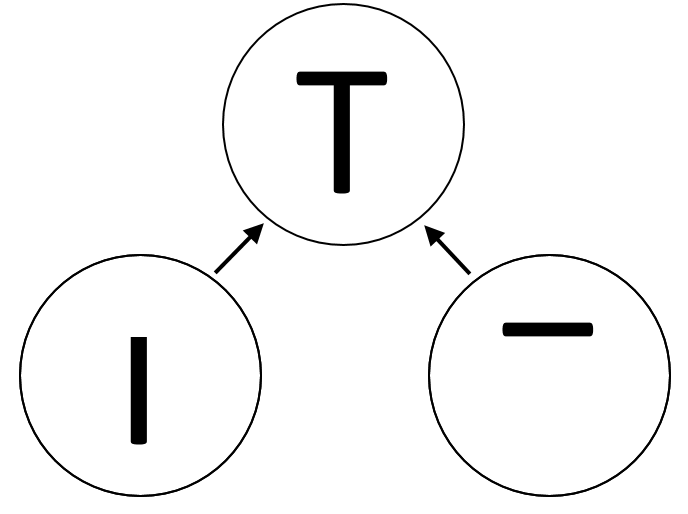
\includegraphics[width=0.3\textwidth]{graphics/compositionality1}
\label{fig:compositionality1}
\caption{Combining two simple features into a more complex feature/composition.}
\end{figure}

In (ref to paper) a hierarchy is built, combining features in a lower layer into more complex features in the layer above it. 
The motivation for using a hierarchy is discussed in section \ref{sec:deep_hierarchies}. 
Three different types of layers is used: 
\todo[inline, author=Michael]{I need a graphic here.. }

\paragraph*{The bottom layer} extracts simple features (edges) from the image. It uses a filter bank\footnote{A filter bank is simple an array of filters that splits the signal into different components. (ref: wikipedia filter bank)}
 consisting of 6 different Gabor filters of different orientation.\footnote{Gabor filters is a combination of a Sinus and a Gaussian distribution that is often used within computer vision for edge detection. (need ref)} 
The filter bank is shown in figure \ref{fig:filterbank}. 
This filter bank is applied directly to the image and features is extracted. 
This is repeated for different image scales, to be make the system robust towards the objects being of different sizes. 
The feature extraction/detection done at this layer is similar to the one of the PVC, namely the area V1. See section \ref{sec:pvc}. 


\begin{figure}[h!] %filterbank  %zoom = 400%
\centering
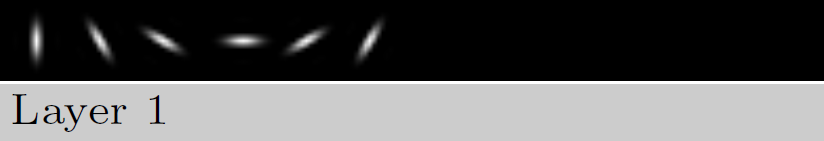
\includegraphics[width=0.4\textwidth]{graphics/layer1_features}
\label{fig:filterbank}
\caption{Filter bank used for feature extraction at layer 1.}
\end{figure}

\paragraph*{Category independent layers} is located just above the bottom layer, and is learned without supervision. In the paper, Layer 2 and 3 is category independent layers.  The features is learned by combining parts from the layer below it (ie. Layer 2 is learned from Layer 1 features, Layer 3 from Layer 2 features etc.). This is described in section \ref{sec:grouping_of_parts}. Examples of of layer 2 and 3 features is shown in figure \ref{fig:layer2+3}. 

The learning of these layers is unsupervised - this means that no input from humans is necessary when the layers are learned. Also, the layers are learned from a set of images containing a variety of objects. 


\begin{figure}[h!] %layer2 + 3  %zoom = 400%
	\centering
\begin{subfigure}[b]{0.3\textwidth}
	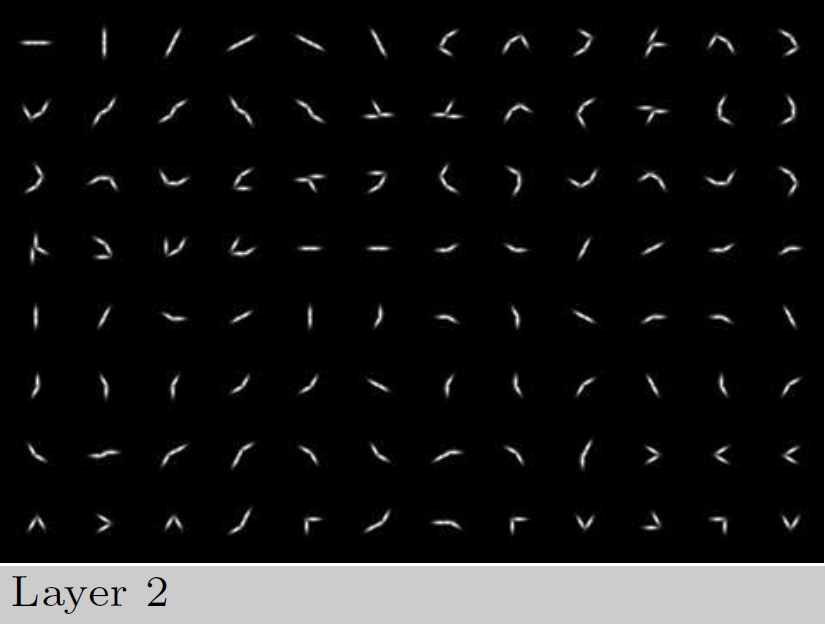
\includegraphics[height=4cm]{graphics/layer2_features}
	%\caption{blabla}
\end{subfigure}
\hspace{1cm}
\begin{subfigure}[b]{0.3\textwidth}
	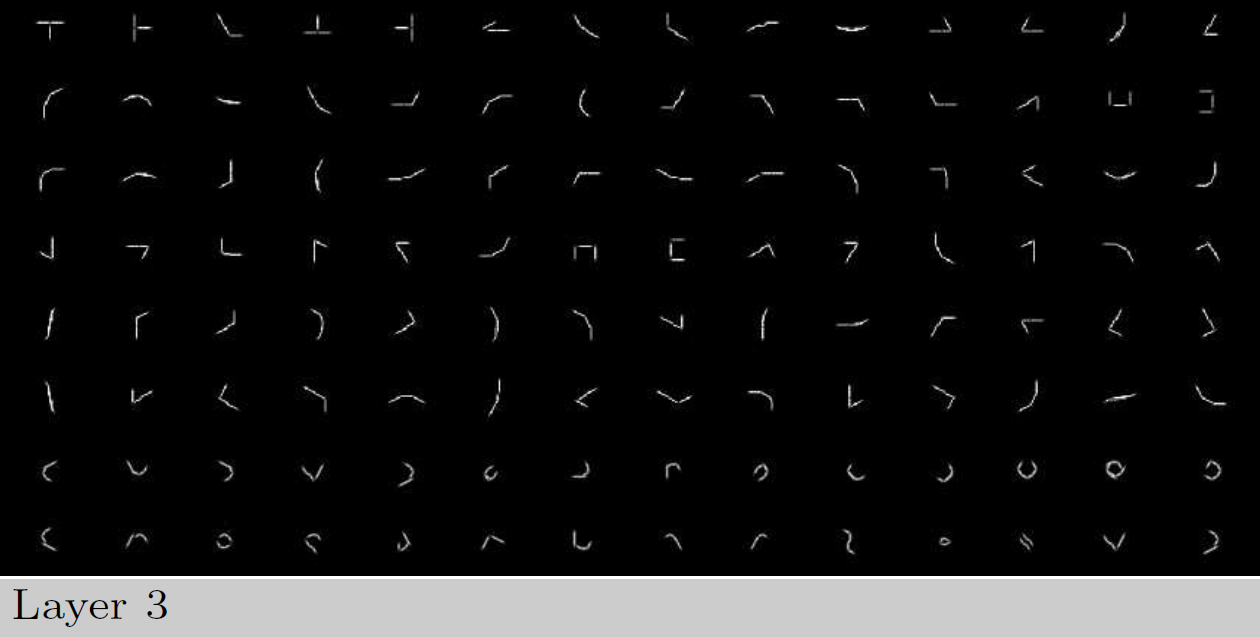
\includegraphics[height=4cm]{graphics/layer3_features}
	%\caption{blabla}
\end{subfigure}

\label{fig:layer2+3}
\caption{Learned features in layer 2 and 3.}
\end{figure}

\paragraph*{Category specific layers} is the highest layers (4 and 5) of the hierarchy. These layers 


\subsection{Grouping of parts}
\label{sec:grouping_of_parts}

